%!TEX root = ../thesis.tex

\chapter{2D Heat Transfer Methodology}
The first step before experimenting with the 3D heat transfer simulation is to understand the simplest form of heat transfer in buildings. This chapter presents the calculation of a 2D section of a single-layer brick wall. Followed by the experimental design, results, and discussion.

\section{Manual Estimation of Heat Flux}
The heat flux calculation for the 2D section shown in \ref{fig:2d2} \textbf{(a)} is as follows:
\begin{equation}
q = -k \frac{dT}{dx}
\end{equation}

where q is the heat flux,
k is the Thermal conductivity, and
$\frac{dT}{dx}$ is the Temperature gradient, which can be found by $\frac{T_2 - T_1}{L}$ over thickness L \cite{heattransfund}. 

Solving for q where k = 1 ${W/m}^2$, 
L = 0.43 m,
$T_1$ = 25.8 \, $^\circ$ \text{C}, 
$T_2$  = 21.1 \, $^\circ$ \text{C}



Substituting the given values:
\[ q = -1 \, \text{W/m}^2 \times \frac{21.1 \, ^\circ \text{C} - 25.8 \, ^\circ \text{C}}{0.43 \, \text{m}} \]
\[ q = 10.93 \, \text{W/m}^2 \]
So, the heat flux \( q \) is \( 10.93 \, \text{W/m}^2 \).





\section{Heat Flux Sensors Experiment}



This section presents a real-time measurement of the 2D brick wall in 359D office located in the Hinman building with a duration of 74 hours using U-value and heat flux sensors as shown in \ref{fig:figexp1} \textbf{(a)} and \ref{fig:figexp1} \textbf{(b)}. Then followed by a 2D simulation section where the same experimental design conditions are implemented in HTflux \cite{HTflux} a 2D heat transfer simulation software. The experiment started on 2024-03-14 at 14:24:15 until 2024-03-17 at 15:24:15. 


\begin{figure}[htb]
    \centering
    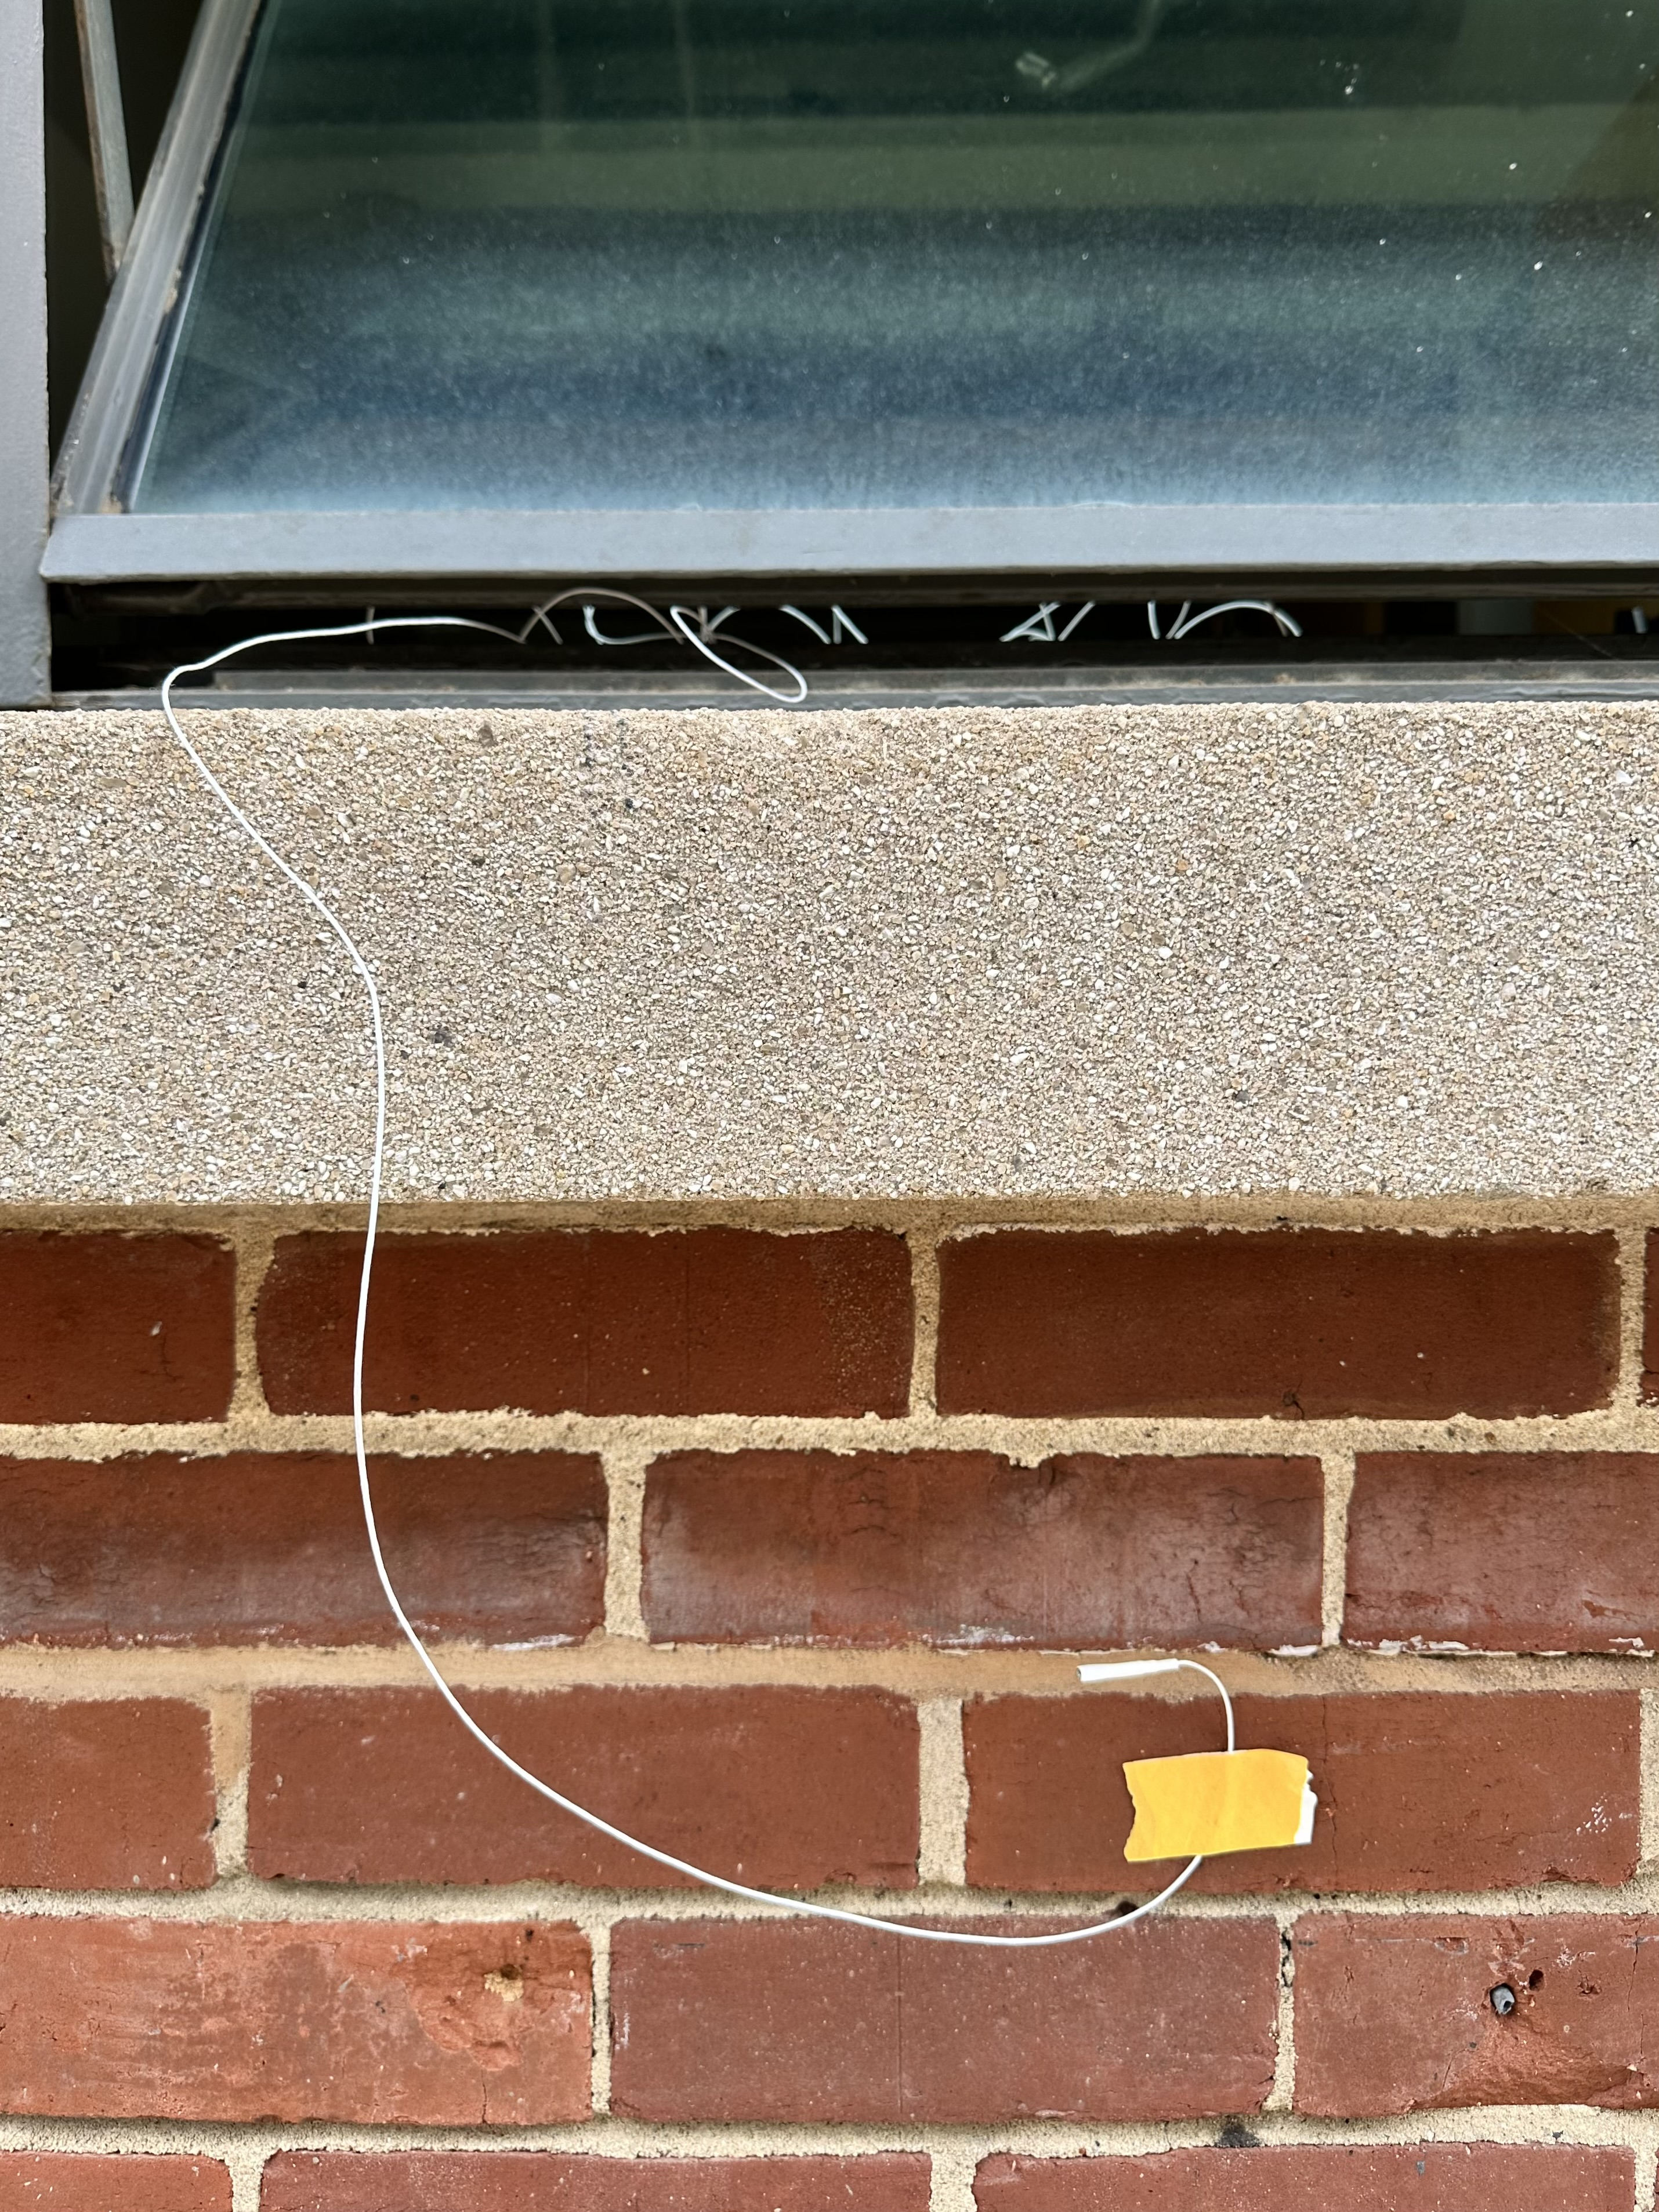
\includegraphics[width=0.495\linewidth]{Figures/expfig1.jpg}
    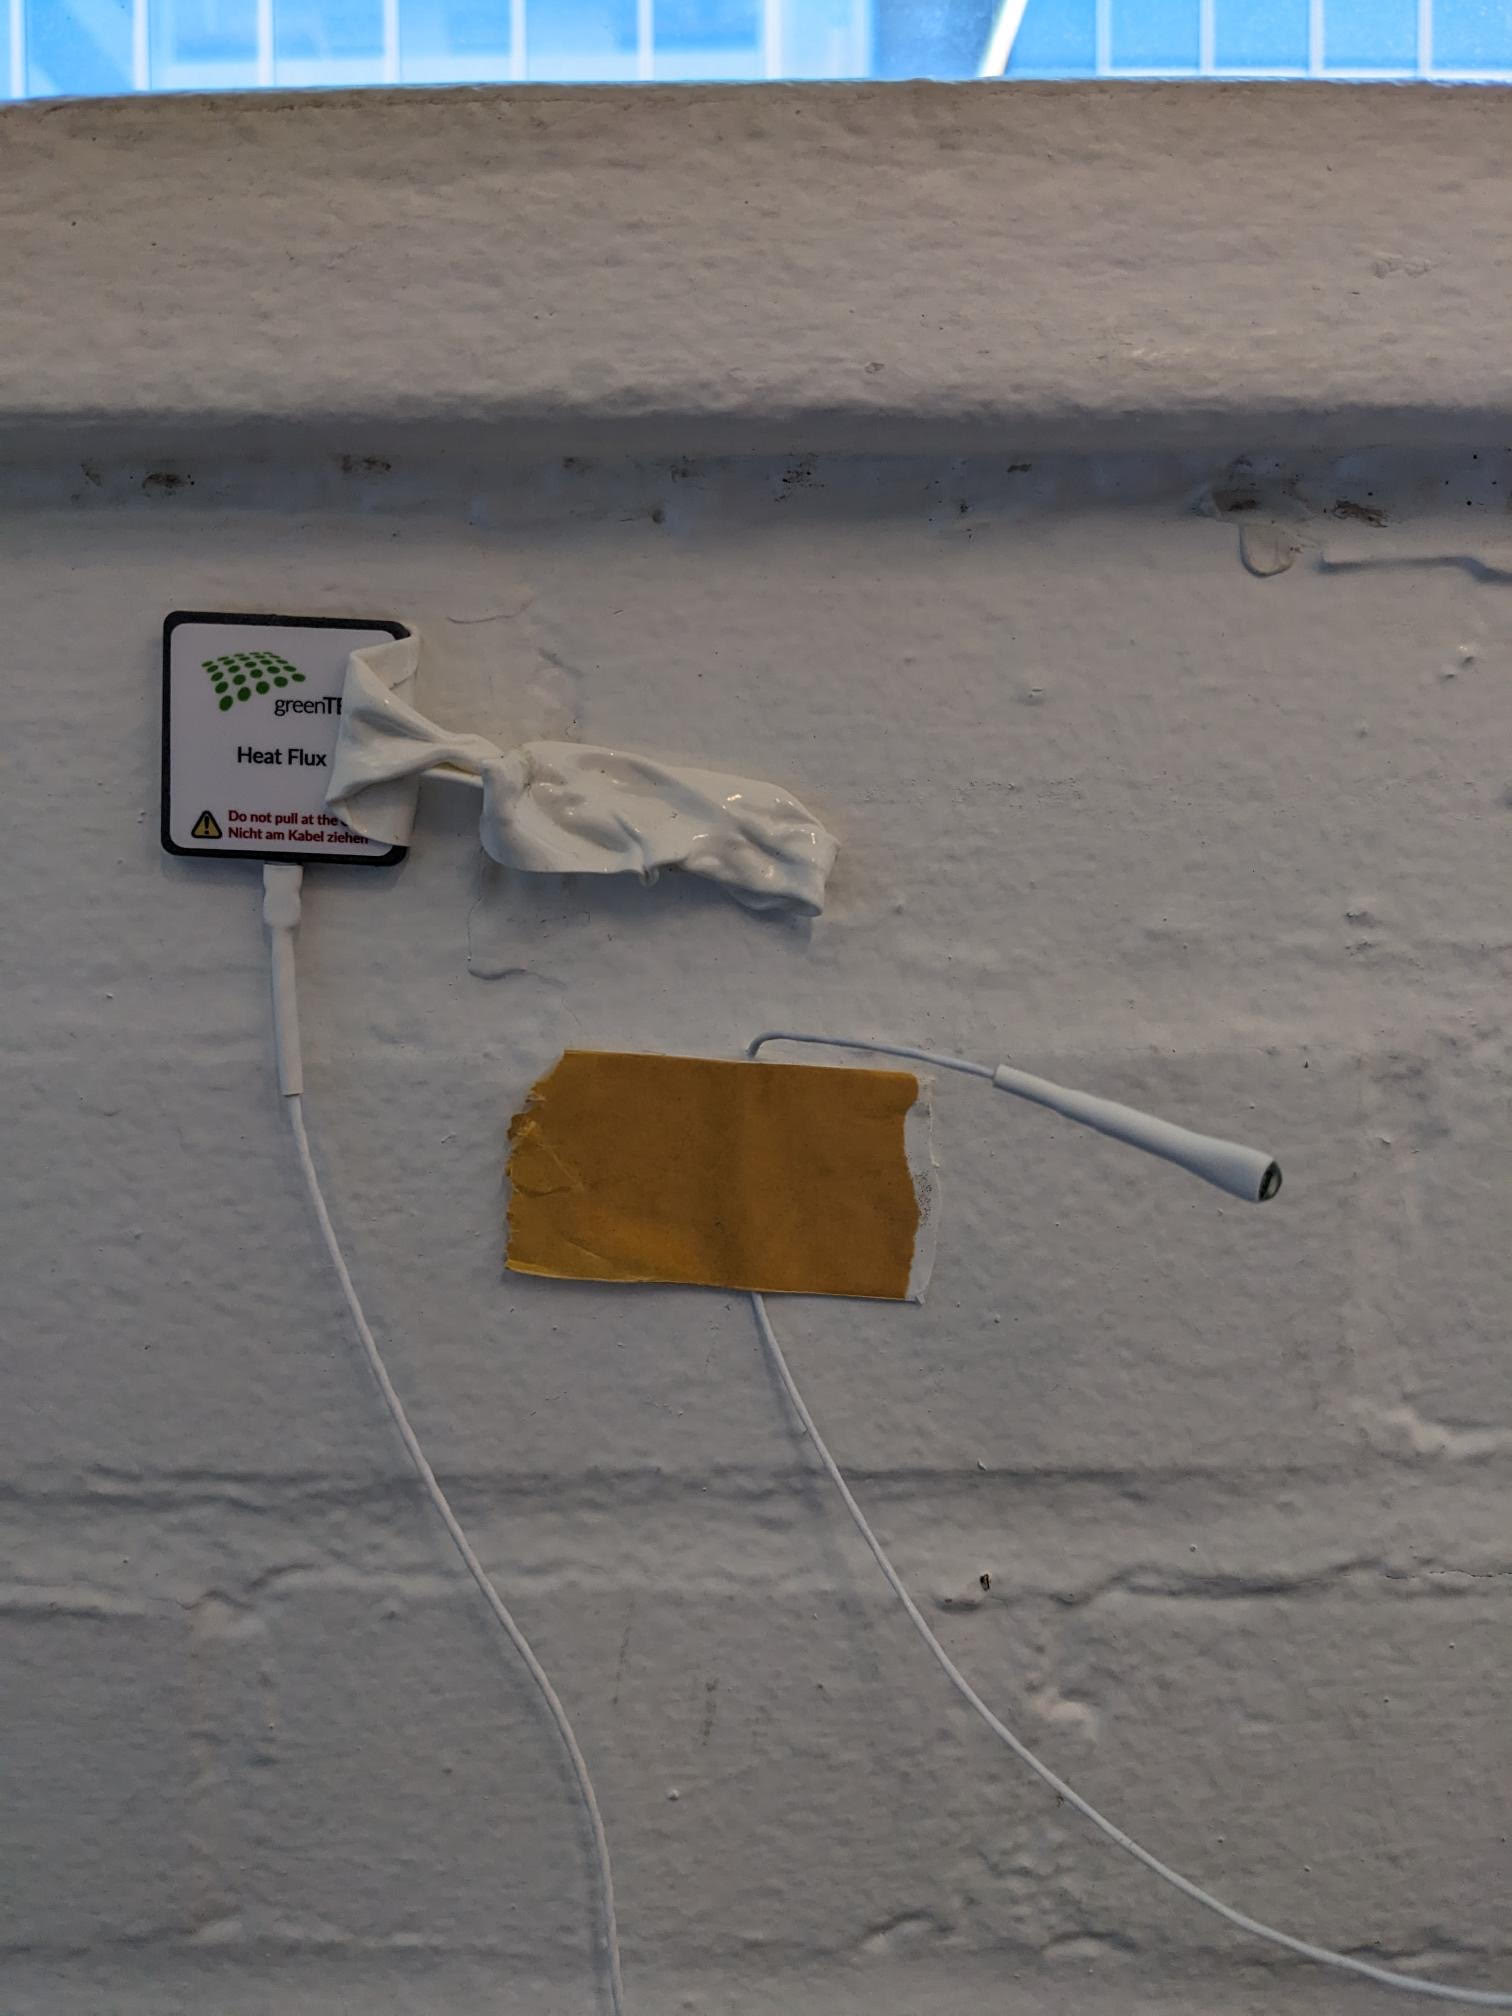
\includegraphics[width=0.495\linewidth]{Figures/expfig2.jpg}

    \hspace{3.5cm}\textbf{(a)}\hfill\textbf{(b)}\hspace{3.7cm}

     \caption[Experimental heat flux measurement setup]{Outdoor heat flux sensors during experimental design. The window was closed as much as possible to avoid interference with the sensor cord \textbf{(a)}. Indoor heat flux sensors during the experimental design \textbf{(b)}.}
   \label{fig:figexp1}
 \end{figure}




 
\subsubsection{Experimental Design}
 Th  measurement device used was the gSKIN® KIT-2615C (calibrated) U-Value and Heat Flux Measurement Kit from GreenTeg  \cite{greenteg} shown in \ref{fig:toolkit} and was purchased by the funding received from The Kendeda microgrant\cite{kendeda}.
 The schematic in \cref{fig:2d2} shows the experimental design setup with the same conditions of k  = 1 ${W/m}^2$ 
L  = 0.43 m,
$T_1$ = 25.8 $^\circ \text{C}$, 
$T_2$  = 21.1  $^\circ \text{C}$ .

\begin{figure}[tbh]
     \centering
    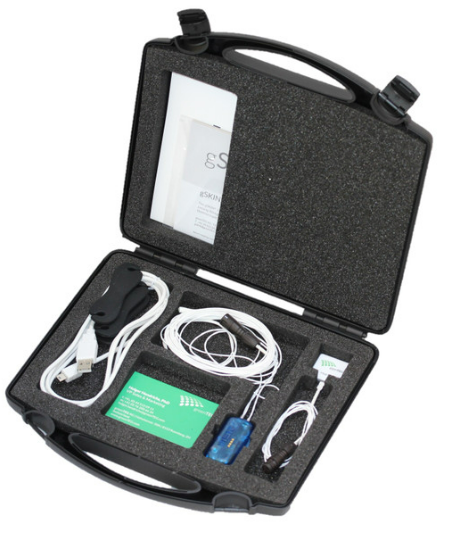
\includegraphics[width=0.5\linewidth]{Figures/greenteg.png}
     \caption[U-value measurement Kit]{The U-Value and Heat Flux Measurement Kit, for details see \cref{tab:u-value-measurement-kit}.}
   \label{fig:toolkit}
 \end{figure}






\subsubsection{Experiment Results}
The chart in \ref{fig:expr} represents the reading results of 74 hours. The final resulting U value = 2.31 ${W/m^2k}$ from the report and the temperatures show compliance with the calculation section above \( q \) is \( 10.93 \, {W/m}^2 \). 
Where U-value from the report = 2.31 ${W/m^2k}$ and 
\begin{equation}
    U = \frac{k}{\text{L}}
      = \frac{1}{\text{0.43}} = 2.33  {W/m^2k}
\end{equation}
Where k = 1 \text{ W/(m²)}, L (thickness) = 0.43. So, \(U_{\text{calc}}\) = \(U_{\text{exp}}\) = 2.31 ${W/m^2k}$ 

\ref{fig:expr} below is a plot report showing the experimental design results of the fluctuations in indoor and outdoor temperature along with the heat flux. From the report, three temperatures from different time steps were selected to be compared with the 3D simulation results. Also, \ref{table2d} shows the comparison of the selected three points, where $T_{val}$ is the experiment's resulting temperature and $T_{sim}$ is the simulation's resulting temperature.

\begin{figure}[htb]
     \centering
    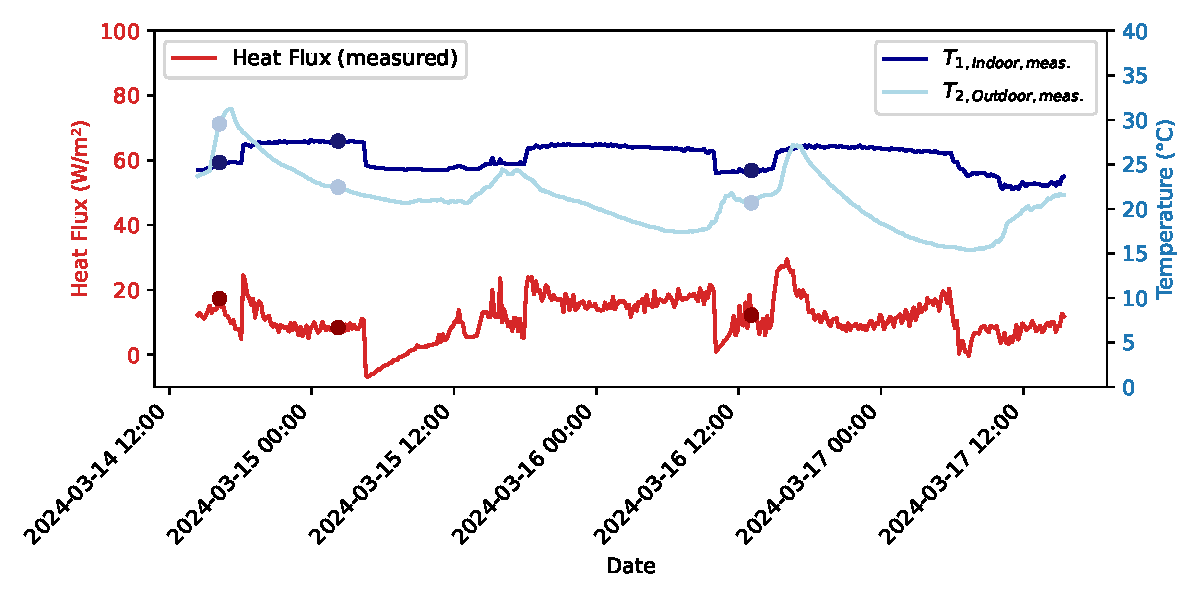
\includegraphics[width=1\linewidth]{Figures/Validation}
     \caption[2D Experimental Report Plot]{The line plots represent the sensor's heat flux and Temperature readings. where the points are the OF simulation results.}
   \label{fig:expr}
 \end{figure}


\begin{table}[tbh]
    \caption{2D Temperature and Heat Flux Comparison}
    \label{table2d}
    \centering
    \begin{tabular}{lrrrrrrr}
        \toprule
        Time                & $T_{1,val,in}$ & $T_{1,sim,in}$ & $T_{2,val,out}$& $T_{2,sim,out}$ & $Q_{val}$ & $Q_{sim}$ \\
        \midrule
        3/14/2024 16:14 & 298.3    & 298.3    & 302.7     & 302.7     & 17.3 & 17.2 \\
        3/15/2024 02:14  & 300.7    & 300.7   & 295.5    & 295.6     & 8.9  & 8.3  \\
        3/16/2024 13:04 & 297.4  & 297.4   & 293.8   & 293.8   & 12.54 & 12.2  \\
        \bottomrule
    \end{tabular}
   
\end{table}

\begin{table}[]
 \caption{2D Results Percentage of error}
    \label{error2d}
     \centering
 \begin{tabular}{l l l}
        \toprule
        Metric & T1 Percentage Error & T2 Percentage Error \\
        \midrule
        Average & 0.0032\% & 0.0102\% \\
        Standard Deviation & 0.0033\% & 0.0176\% \\
        \bottomrule
    \end{tabular}
\end{table}


\begin{figure}[tbh]
  \centering
  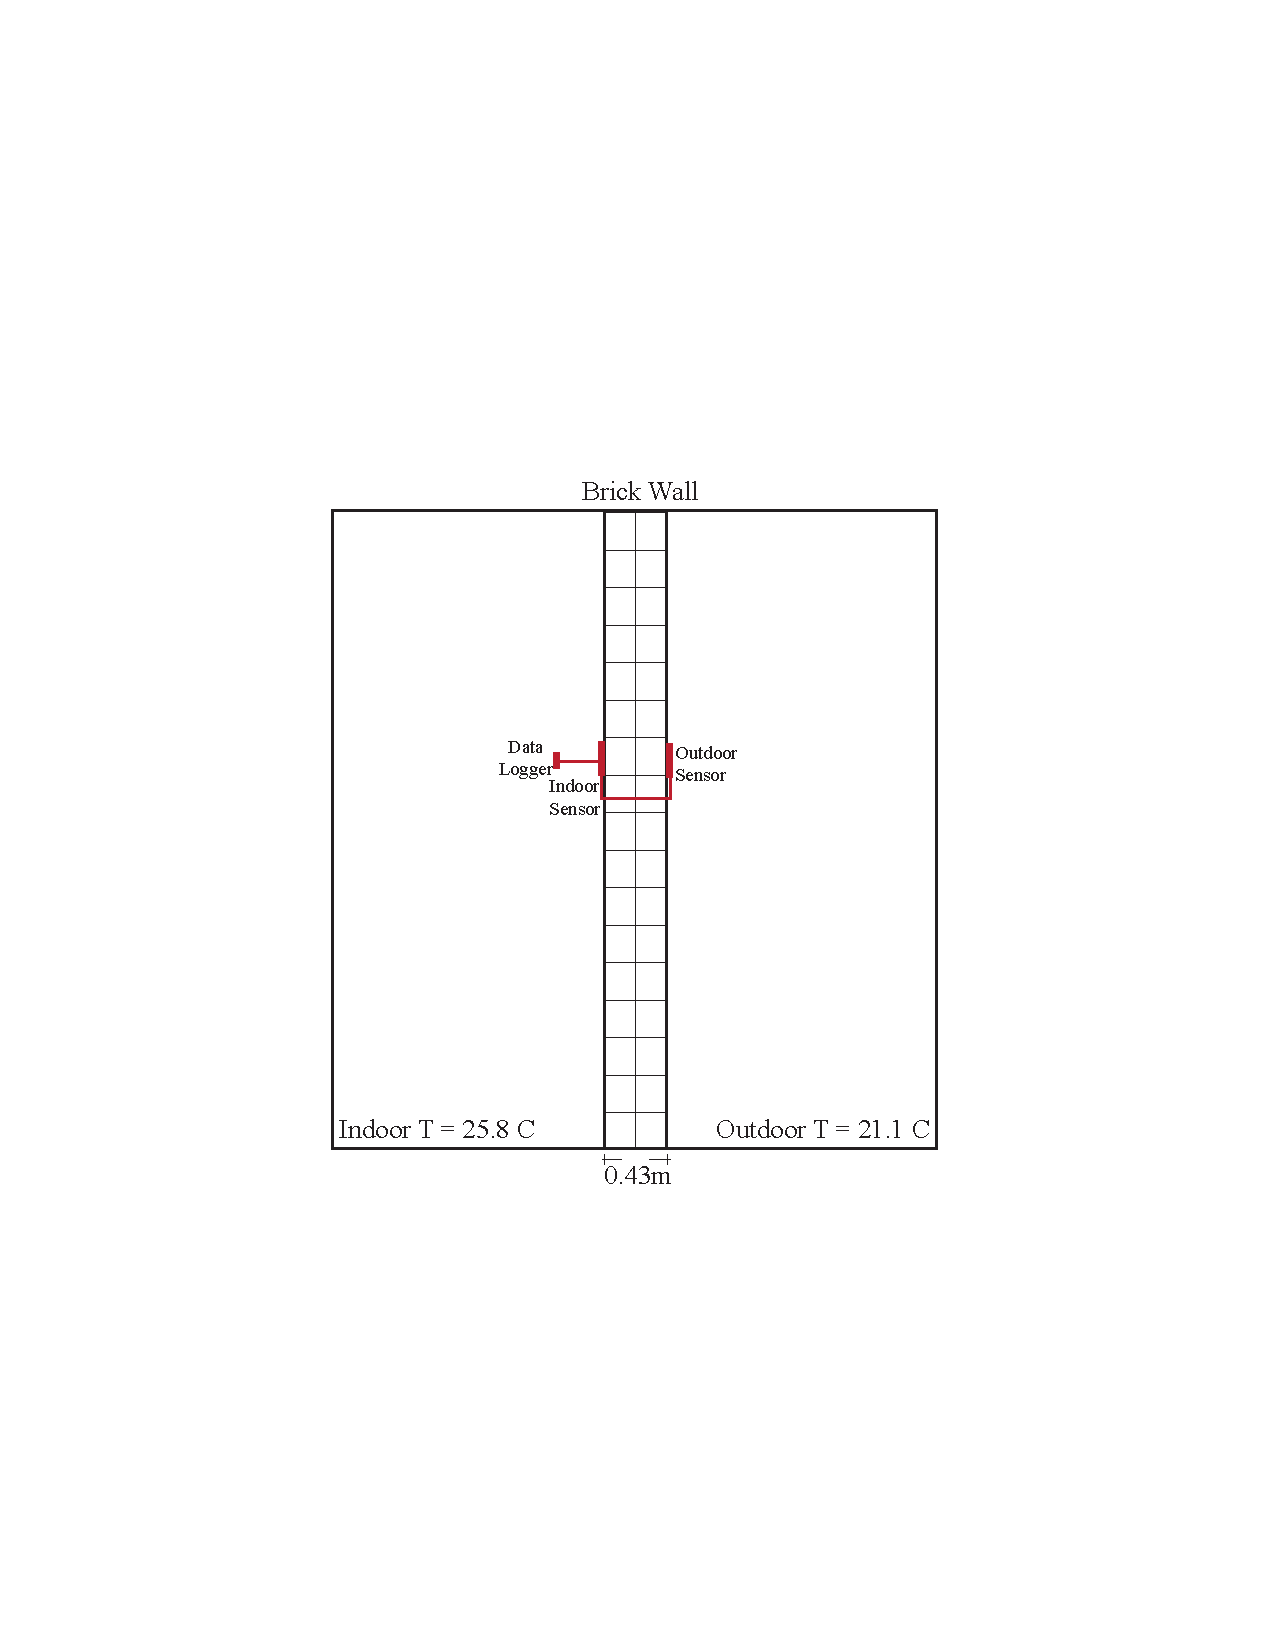
\includegraphics[trim=5.6cm 7.5cm 5.3cm 8cm, clip, width=.7\linewidth]{Figures/2dsection2.pdf}
\caption[2D Section and Setup]{Experiment setup for the 2D brick wall.}
\label{fig:2d2}
\end{figure}




















\section{Simulation}
\todo{add subsections here that make very clear that the first simulations are done with OpenFOAM, the others are done with HTFlux}

After successfully finding and ensuring the compliance of the heat flux in the two methods, which are the calculation and the experiment, the final method uses a 2D heat transfer simulation, HTFlux \cite{HTflux}. The same brick wall with the same boundary conditions is constructed in the software as shown in \ref{2dconst} \textbf{(a)} which shows the materials and the boundary condition and \textbf{(b)} represents the 2D simulation results where the resulting heat flux = \( q \) is \( 10.91 \, {W/m}^2 \) as expected.





\begin{figure}[tbh]
\begin{minipage}{0.45\textwidth}
  \centering
  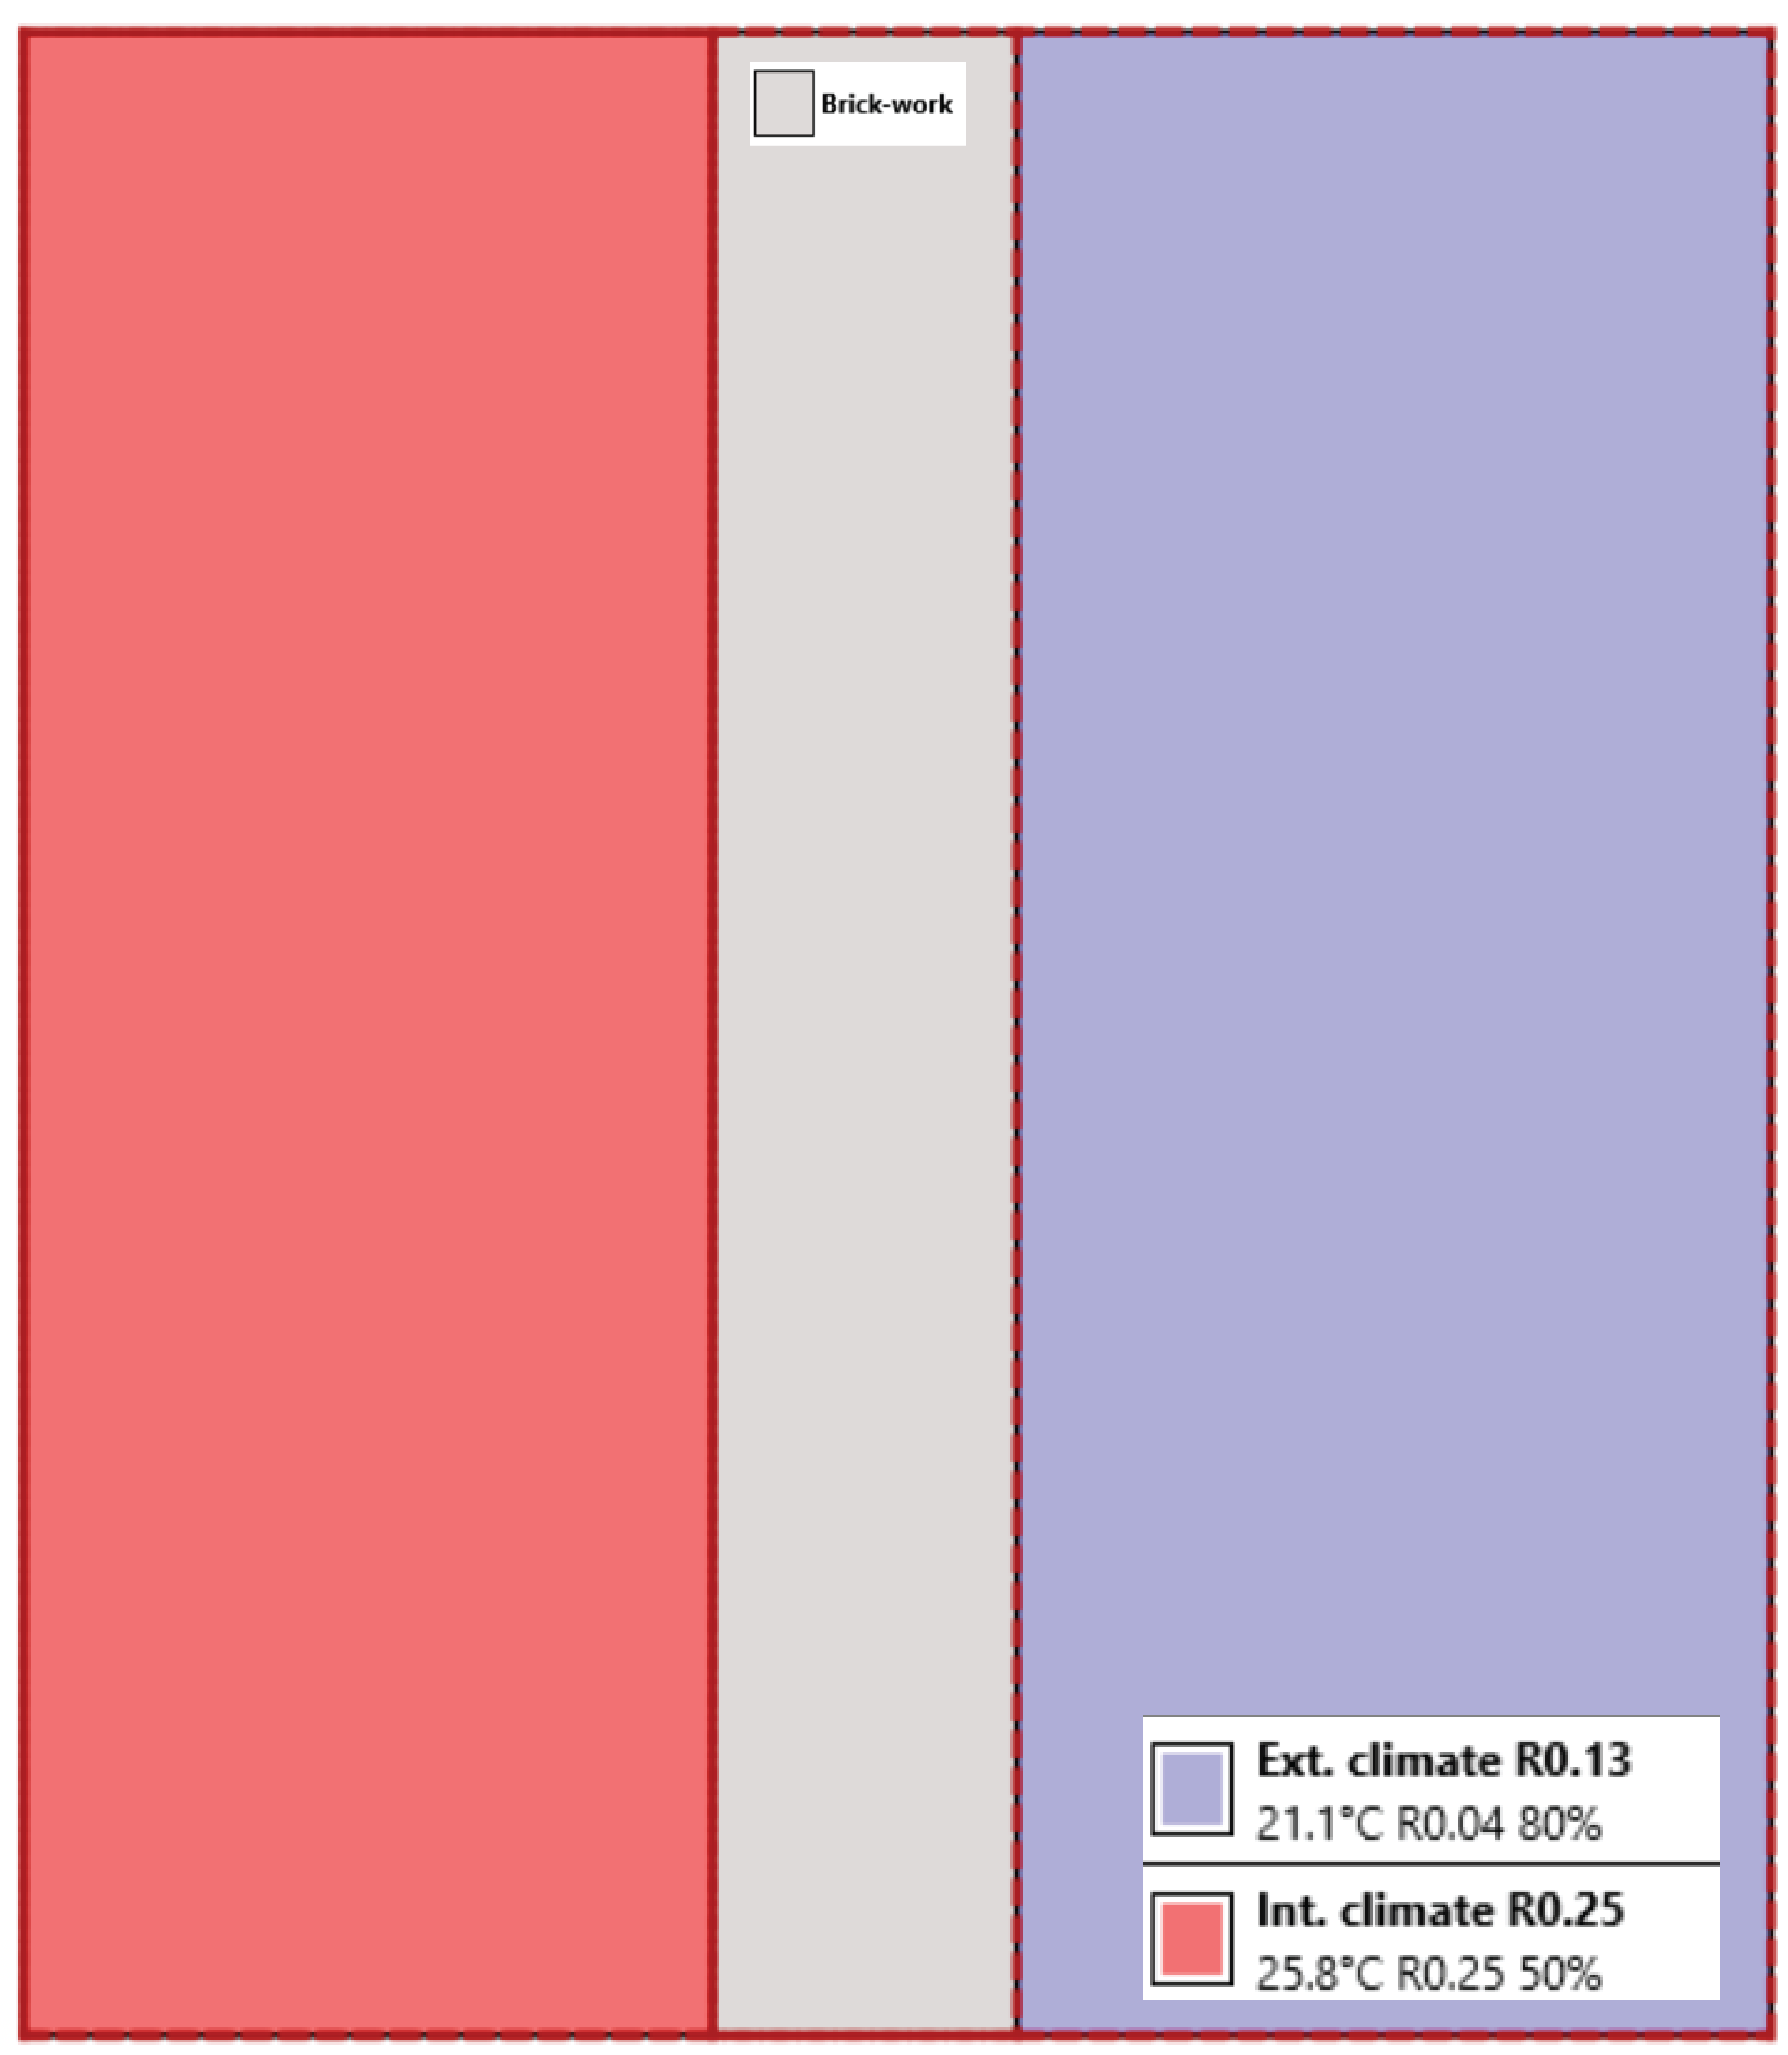
\includegraphics[width=\linewidth]{Figures/2dconst.png} 
  \caption*{\textbf{(a)} The simulation boundary conditions from HTFlux}
\end{minipage}%
\hspace{0.1\textwidth}
\begin{minipage}{0.45\textwidth}
  \centering
  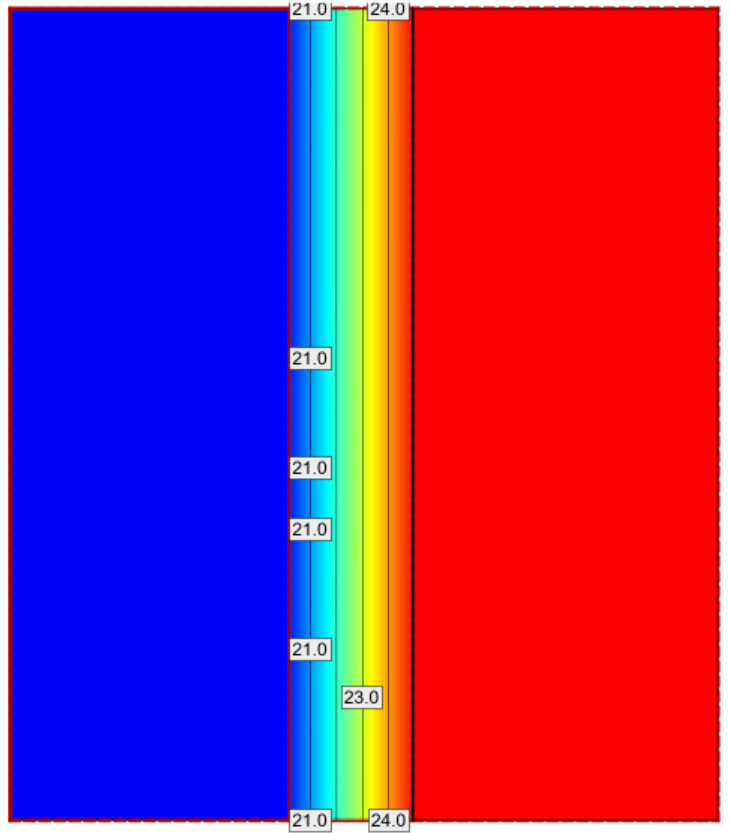
\includegraphics[width=\linewidth]{Figures/2dsim.png} 
  \caption*{\textbf{(b)} The brick wall temperature gradient results from HTFlux}
\end{minipage}
\caption{2D HTFlux Boundary conditions and Resulting heat flux of \( 10.91 \, {W/m}^2 \)}
\label{2dconst}
\end{figure}


\section{Discussion}
This section successfully presented the resources to calculate the heat flux of a 2D brick wall using three methods, which are by calculation, using sensors, using 2D simulation software where the heat flux q, respectively, = \( 10.93 \, {W/m}^2 \), \( 10.93 \, {W/m}^2 \), and \( 10.91 \, {W/m}^2 \). However, the gap of 3D heat transfer simulation is still missing. Thus, chapter 3 showcases the workflow of a free 3D heat transfer simulation.